\chapter{Realisation and Result}
This chapter describes the model, the architecture and the modules of MAELAB (Morphometric with Automatically Extraction of Landmarks) software. The first part is description about model as well as the packages in program. Then, we give the modules in program, class diagram and explain about it.
\section{Software architecture and the packages}
The MAELAB software mainly includes two packages: \textbf{MAgIS} package and \textbf{Morphometry} package. The \textbf{MAgIS} package contains the methods to segment images and construct the interface of program. This package was finished by NGUYEN Hoang Thao. The \textbf{Morphometry} package is the new one, it contains the implementations to estimate landmarks automatically. Besides, we also use the method provides by OpenCV library(OpenCV library) and Qt framework (Qt Framework package) (see in figure \ref{fig:42}).
\begin{figure}[h!]
\centering
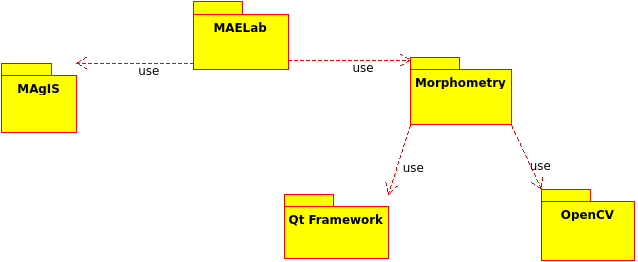
\includegraphics[width=0.8\textwidth]{./images/packages}
\caption{The packages of program}
\label{fig:42}
\end{figure}~\\
\section{The modules of software}
The software includes four main modules corresponding to four processes to estimate the landmarks: segmentation module, pairwise geometric histogram (PGH) module, probabilistic Hough transform (PHT) module and landmark detection module. Besides, the environment module provides the common classes. The classes in environment module can be used in all modules of software (figure \ref{fig:41}).
\begin{figure}[h!]
\centering
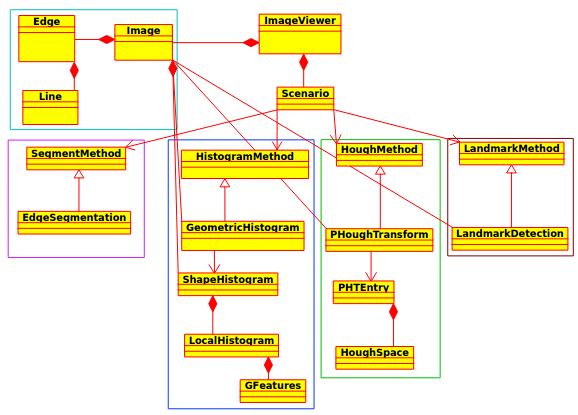
\includegraphics[width=0.8\textwidth]{./images/modules}
\caption{The modules of program with main classes}
\label{fig:41}
\end{figure}
\subsection*{Environment module}
Environment module contains the classes used to describe the information presented for object in image: \texttt{Image}, \texttt{Edge}, \texttt{Line}. The classes in this module can be used for all modules in MAELab.
\subsection{Segmentation module}
The segmentation module implements the pre-process image and extracts the edges from image. The main classes in this module includes \texttt{SegmentMethod} class and \texttt{EdgeSegmentation} class. \texttt{SegmentMethod} class is designed as an abstract class of segmentation, this is the connecting port between this module and other modules. Class \texttt{EdgeSegmentation} extends from \texttt{SegmentMethod}, it implements the method to pre-process and extract the features from image. 
\subsection{PGH module}
The PGH module provides the ways to implement the constructor of PGH and compute the measure metric between PGHs. In PGH module, class \texttt{HistogramMethod} is a abstract class, it provides the method to construct the PGH of an image. Its methods was implemented in \texttt{GeometricHistogram} class (\texttt{GeometricHistogram} extends from \texttt{HistogramMethod}). Basically, the method to construct the PGH come from other classes. Class \texttt{GeometricHistogram} uses these methods to finish the implementation from abstract class. In addition, \texttt{GeometricHistogram} also provides different methods in PGH such as: compute the measure metric by Bhattacharya metric, Chi-squared metric or Intersection metric; change the accuracy of PGH.
\subsection{PHT module}
PHT module finishes the works in estimation stage. The main methods of PHT module stay in \texttt{PHoughTransform} class. It is a class extended from \texttt{HoughTransform} class, an abstract class. Besides the method extends from abstract class, \texttt{PHoughTransform} also implements the methods when we apply the probabilistic Hough transform as described in previous chapters.
\subsection{Landmark detection module}
The landmark detection module used to implement the methods to refine the estimated landmarks from estimation stage. It includes an abstract class, \texttt{LandmarkMethod}, and an implement class which extends from abstract class, \texttt{LandmarkDetection} class. \texttt{LandmarkDetection} class implements the methods to refine the estimated landmarks and compare the accuracy between the estimated landmarks and manual landmarks.

The figure \ref{fig:43} shows class diagram of this software. The \textbf{main} methods located in the \texttt{ImageViewer} class, where contains all functions of the software and connects with the \textbf{MAgIS} package. The connecting between the software and the modules made via \texttt{Scenario} class. To represent the information of image, we use the classes: \texttt{Line}, \texttt{Edge}, \texttt{Image}. For each main modules in program, we have the abstract classes, implementation classes and the support classes. \\
\begin{figure}[h!]
\centering
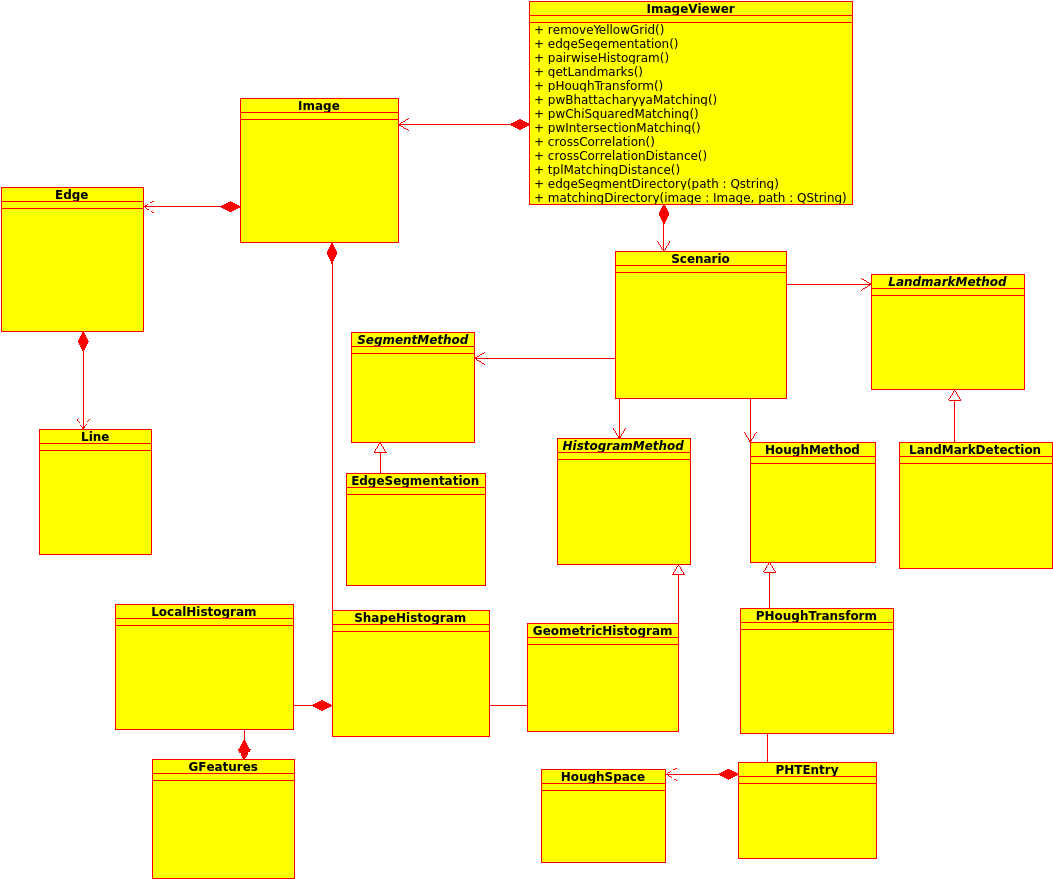
\includegraphics[width=1.1\textwidth]{./images/main}
\caption{The class diagram of program}
\label{fig:43}
\end{figure}
\subsection*{Environment classes}
The \textit{environment classes} describes information about the classes which describe the geometric objects that can be represent the image and the method to remove the yellow grid on the images.

The \texttt{Line} class descibes the information of a straight line and its method, such as: get the length of line, compute the perpendicular distance from a point to line, find the intersection between two lines, compute the angle between two lines, find the parallel line with this line.

The \texttt{Edge} class uses to present a curve and the methods with edge. An edge can be presented by a list of lines or a list of points. The important methods in \texttt{Edge} class are \texttt{breakEdge()} and \texttt{segment()} method. It used to break the edge into approximate lines based on the list of point constructed edge.

The \texttt{Image} class presents the information of an image such as file name, list of edge extracted from it. Besides, \texttt{Image} class also provides the methods to get the file name of image, compute the histogram of image, get the PGH of image, read its landmarks from a file, etc.
\subsection*{The abstract classes}
The abstract classes contains the abstract methods correspondence with the main modules of program. They provide the abstract methods which was implemented in the inherit classes. As introduce in previous section, the abstract classes include: \texttt{HistogramMethod} class, \texttt{SegmentMethod} class, \texttt{HoughMethod} class, \texttt{LandmarkMethod} class.
\subsection{Edge segmentation }
\textbf{Edge segmetation} includes classes used to segment an image. Besides, the classes construct the edge which is described in previous section such as \texttt{Line, Edge,...}, we also provide the access methods for other classes.

The \texttt{EdgeSegmentation} class provides the methods such as obtaining the lines from an image, present the result of segmentation or applying the segmentation on an image folder. The methods in \texttt{Edge segmentation} are:
\begin{itemize}
\item Extract the approximate lines of object in an image,
\item Extract the approximate lines of object in each image in a folder.
\end{itemize}
\subsection{Pairwise Geometric Histogram}
This section describes the classes used to construct the PGH and compare the measurement of them.

\texttt{GFeatures} class contains the relative information of the objects in PGH such as angle, minimum distance and maximum distance. It provides the methods to get and set the relative information.

\texttt{LocalHistogram} class is constructed to contain the information when computing the PGH of a line in object. The chosen lines as reference lines, the local histogram is constructed based on recording the relating between reference line and other lines in object. Besides, it has the methods for the user to change the accuracy, such as the angle accuracy or the distance accuracy.

\texttt{ShapeHistogram} class constructs the PGH for an object. It is constructed by on combing all PGH of the lines in an object. It also provides the methods to compute the measured distance between the pairwise geometric histograms by a matching method. The methods in this class includes:
\begin{itemize}
\item Construct the PGH for an image,
\item Construct the matrix to save the PGH result,
\item Compute the measured distance between the two PGHs based on \textit{Bhattacharyya}, \textit{Chi-Squared} or \textit{Intersection} metric.
\end{itemize}

\texttt{GeometricHistogram} class provides the access ways for other classes. By usign this class, user can compute the pairwise geometric histogram of an image and calculate the distance between the pairwise geometric histograms.
\subsection{Estimate the global pose (Probabilistic Hough Transform)}
This section describes the classes use probabilistic hough transform to estimate the model image from a scene image. In particular, it is estimating the reference landmarks on the scene image.

\texttt{HoughSpace} class contains the information about the angle and distance from a line to a reference point. These information is recorded to construct the accumulator when we apply the Probabilistic Hough Transform.

\texttt{PHTEntry} class presents each entry when constructing the reference table in the training process. Each entry contains the pair of lines and its information about angle and distance to a reference point.

\texttt{PHoughTransform} class describes the main process when we apply the probabilistic hough transform to estimate the landmarks. It includes the methods to construct the reference table, find the reference point in scene image and estimate the landmarks. Besides, it also provides the methods to estimated the landmarks of an image on the directory of images.
\subsection{Refine the landmarks}
\texttt{LandmarkDetection} class provides the methods to refine the estimated landmarks by probabilistic Hough transform. It also implements the cross-correlation technique to match the model and the image and provides the methods to compare the estimated result with the original result (by comparing distance between the landmarks).